\chapter{\IfLanguageName{dutch}{Stand van zaken}{State of the art}}
\label{ch:stand-van-zaken}

% Tip: Begin elk hoofdstuk met een paragraaf inleiding die beschrijft hoe
% dit hoofdstuk past binnen het geheel van de bachelorproef. Geef in het
% bijzonder aan wat de link is met het vorige en volgende hoofdstuk.

% Pas na deze inleidende paragraaf komt de eerste sectiehoofding.

Dit hoofdstuk bevat je literatuurstudie. In dit onderdeel zal er diep in gegaan worden op het onderwerp. Delen van het onderwerp worden grondig onderzocht om later tot een conclusie te komen. 

\section{Microservices}
\subsection{Definitie}
Het artikel van \textcite{Mauersberger2017} gaat over hoe grotere bedrijven omschakelen naar microservices. Bij een verandering binnen een monolithic architectuur, werd er een heel nieuwe versie van de architectuur uitgebracht. Een verandering bracht een hoop extra werk mee. De definitie die te vinden is in dit artikel, gaat als volgt: "A method of developing software applications as a suite of independently deployable, small, modular services in which each service runs a unique process and communicates through a well-defined, lightweight mechanism to serve a business goals.". Als je de definitie leest, zie je drie onderdelen. Het eerste onderdeel vertelt hoe een microservice in elkaar zit. Het is een onafhankelijke, kleine, modulaire services. Deze service communiceert op een eenvoudige manier. Dit is een tweede eigenschap van een microservice. De derde eigenschap omvat dat een microservice wordt gemaakt in functie van een requirement uit de business. Het doel van microservices is de problemen die te vinden zijn bij een monolithic kunnen verholpen worden met microservices. De vorige definite legde uit wat microservices zijn. Dit artikel zegt waar men microservices kan plaatsen. Er is dus één groot framework. Daar zitten meerdere onafhankelijke services in.
\begin{figure}[h]
	\caption{Een monolithic architectuur naast een microservice architectuur.}
	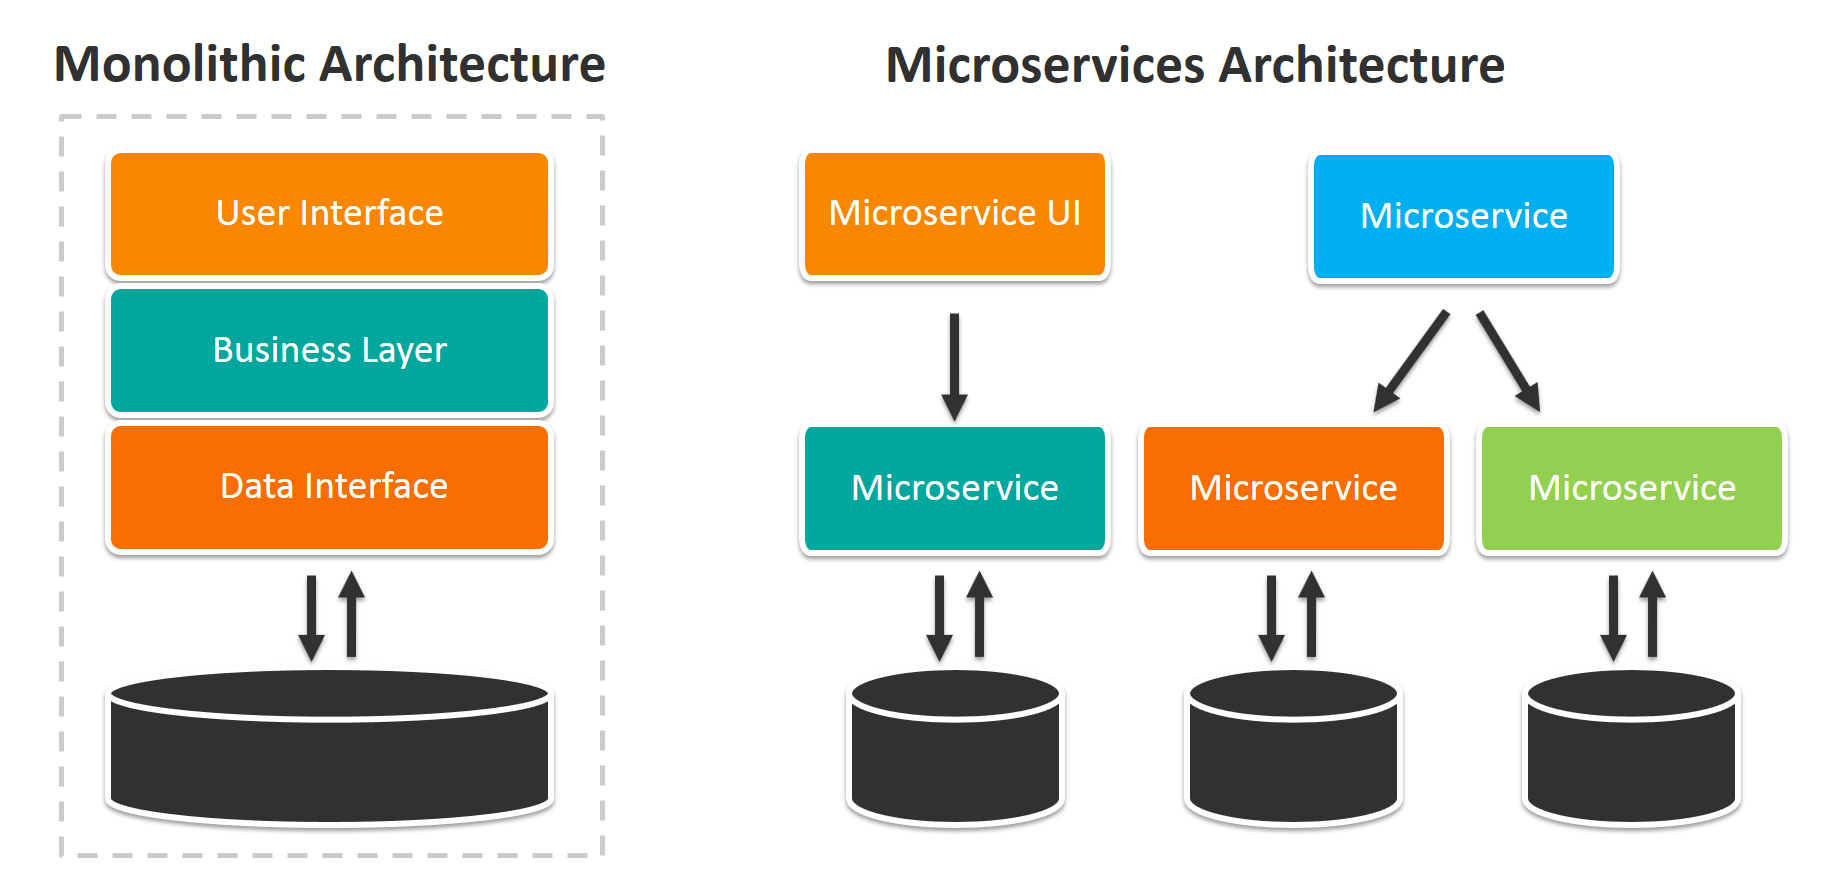
\includegraphics[width=10cm]{microservices-vs-monolithic.jpg}
	\centering
\end{figure}
Figuur 2.1 is afkomstig uit artikel \textcite{Watts2018}.
Zoals te zien in figuur 2.1 is er een groot verschil tussen een monolithic architectuur en die van een microservice. Bij een monolithic communiceren alle deeltjes van een applicatie met een grote databank of datastore. Dit wordt goed weergegeven in de linkerkant van de foto. Aan de rechterkant van de foto is een voorbeeld te zien van een microservice architectuur. Daar is duidelijk te zien dat elke microservice een eigen databank/datastore heeft. Voor een functionaliteit wordt een microserives aangemaakt, die dan nog eens apart een databank voor zich krijgt. 
\textcite{series2018} bestaat uit elf verschillende onderdelen. Eerst wordt er uitleg gegeven over wat microservices zijn. Hun definitie voor microservices is volgende: "A software architecting pattern that allows software to be developed into relatively small, distinct components. Each of the components is abstracted by an API(s) and provides a distinct subset of the functionality of the entire application". Ook hier zien we weer het puntje passeren dat een microservice een klein componentje is van een groter geheel. Die eigenschap wordt heel hard benadrukt. Na het uitleggen van microservices, schrijven ze ook over hoe microservices zo scalable zijn. Ook lichten ze toe hoe belangrijk API's zijn binnen een microservice architectuur. Er wordt ook gepraat over de verschillen tussen een monolithic architectuur en een microservice architectuur. 
\subsection{Het belang van microservices}
Er wordt vaak Agile gewerkt. Dat vraagt na twee weken een afgewerkt stukje software. Bij een monolithic kan het aanpassen van een deeltje, veel werk vragen. Microservices spelen daar gemakkelijk op in. Die technologie legt niet heel het framework plat als er deeltjes moeten bij gecodeerd worden. Microservices kunnen sneller inspelen op de Agile analyse/ontwikkel methode.
\textcite{series2018} haalt aan dat microservices van belang zijn bij het scalen van software.
In het artikel van \textcite{RDX2016} worden er verschillende eigenschappen aangekaart. Microservices moeten een doel in de business vervullen. Naast dit, zorgt microservices er ook voor dat bescherming eenvoudig wordt. Het is belangrijk om te zorgen dat er bescherming is per microservices. Dit gebeurt best op een uniforme manier. Er kan wel veel gezegd worden over hoe broodnodig microservices zijn maar ze laten deployen en dan er niet meer naar omkijken, zal zeker geen problemen oplossen. Ook na het opzetten en laten werken van een microservices moet er gemonitord worden wat er gebeurt. 
Het artikel van \textcite{Watts2018} geeft het belang van een microservice goed weer. Microservices beschermen het gehele systeem, bij een goede implementatie. Ze maken het gebruik van de Agile methode, ook eenvoudiger dan bij een monolithic. Met deze technologie is het eenvoudiger om een aanpassing te testen en te onderhouden. Niet de volledige architectuur moet opnieuw getest worden bij een aanpassing. Als team A een aanpassing doet aan hun microservice, zullen de andere teams geen hinder ondervinden. 
\subsection{Algemene aanpak om microservices te implementeren}
Het interessante artikel van \textcite{Benetis2016} over een 6-stappen plan om microservices te implementeren.
De eerste stap is het bepalen van de business requirements die de microservices zal bedienen. Dit is ook een van de belangrijkste redenen om microservices te gaan gebruiken. Het voldoen aan de business requirements. 
\subsection{De voordelen en nadelen van microserivces}
In het artikel van \textcite{series2018} wordt er veel lofzang gedaan over microservices. Het gebruik van microservices zou ervoor zorgen dat de architectuur flexibeler wordt. Er kunnen microservices hergebruikt worden. Dankzij microservices is het hermodeleren, implementeren van nieuwe technologieën, ... 
Kleinere deeltjes zijn gemakkelijker te documenteren. De snelheid van microservices zijn een groot pluspunt.
\textcite{Watts2018} geeft enkele voordelen van een microservice. Een developer is onafhankelijk. Ze hebben vrijheid. Ook het scalen van een microservice is veel eenvoudiger. Dit komt door dat microservices minder resources nodig hebben dan een volledige monolithic. Een ander voordeel is bij het falen van een microservices, de andere microservices er geen last van zullen hebben. Dit komt door hun onafhankelijkheid. 
\subsection{Voorbeelden}
In dit deeltje zal je meer te weten komen over hoe grote technologische bedrijven microservices toepassen en hoe ze naar deze technologie zijn overgeschakeld.
Een term die hier vaak zal gebruikt worden, is een monolithic. Dit is de tegenhanger van microservices. Sommige zweren bij monolithic en anderen hebben gouden woorden voor microservices. De beslissing om één van de twee technieken te kiezen, ligt bij wat je precies nodig hebt. Wat de business nodig heeft. 

\subsubsection{Amazon}
\textcite{Mauersberger2017} gaf een voorbeeld waarom Amazon overstapte. Zoals veel grote bedrijven is Amazon begonnen met een grote monolithic. Een van de nadelen die Amazon ondervond aan deze technologie is de moeilijkheid van het inschatten van de zwaarte op de servers. Daardoor verloor Amazon veel geld en was er nood aan herstructurering.
\textcite{Fulton2015} legt ook uit waarom Amazon is overgeschakeld. Het blijkt dat Amazon in 2001 de grootste monolithic was in de retail business. Doordat Amazon een snel groeiende onderneming was, werd de monolithic architectuur heel ingewikkeld. Amazon hun aanpak was, gooi wat je hebt niet weg maar maak het eenvoudiger. 
\subsubsection{Apple}
\subsubsection{Facebook}
\subsubsection{Netflix}

\section{Order-to-cash proces in SAP}
\subsection{Definite}
\textcite{Obrien2017} geeft aan dat een order-to-cash bestaat uit processen met business requirements. Dit proces start bij het plaatsen van een order en eindigt bij het innen van het geld. Het proces is in de grote lijnen hetzelfde. Het snel doornemen van het proces, geeft een vertekend beeld. Elk deeltje van dit proces heeft moeilijkheden en uitdagingen. 
Dit proces is heel belangrijk voor bedrijven. Het is de core van de business. Bij een slechte implementatie, kan je klanten verliezen of geld verliezen. 
\subsection{Technologie}
\subsubsection{Onderdelen van een order-to-cash proces}
Er zijn vier grote onderdelen, namelijk:
\begin{itemize}
	\item Voor-verkoopsactiviteiten.
	\item Het order proces.
	\item Order afwerking.
	\item Betaling.
\end{itemize}
Bij de voor-verkoopsactiviteiten verstaan we het contact dat moet worden gemaakt worden met klant. De klant moet overtuigd worden van het product. Na contact komt er al dan niet een offerte. Soms kan er ook van contact rechtstreeks naar een order gaan. 
Het orderproces bevat maar één onderdeel namelijk: de sales order. 
Binnen de order afwerking valt het leveren van goederen, het verzenden van goederen.
\subsubsection{Wat biedt SAP zelf aan voor microservices}
\subsection{Een order-to-cash proces vanuit de business}
\subsection{Het proces afstemmen met de business}

\section{Requirements van de business}

